% !TEX root = ../main.tex
\section{Empirical Study}
\label{sec:rfs-experiments}
We study \gls{rfs} on two datasets and tasks. The first data consists of researcher reading behavior from the arXiv; the semi-synthetic task is to recommend documents to scientists. The second is crowdsourced food consumption data from a diet tracking app, and the task is meal recommendation. On both benchmarks, models in the \gls{rfs} class outperform several baseline methods. The permutation-invariant models we compare to are described in \Cref{sec:models}, and the hyperparameters used are described in \Cref{sec:appendix-empirical}. To show the relative ease of implementation of \gls{rfs} we give example code in \Cref{sec:code}.\footnote{Full source code is available at \url{https://github.com/altosaar/rankfromsets} for reproducibility.}

\paragraph{Recommending Research Papers.} We benchmark \gls{rfs} on data of scientists reading research papers on the arXiv, where the goal is to recommend papers to scientists. This is a semi-synthetic task: it uses real-world data, but the item side information (article abstracts) is not set-valued. Nevertheless, document recommendation is a standard benchmark to study whether \gls{rfs} performs well in settings outside its target purview of meal recommendation. The arXiv data represents one year of usage (2012) and consists of $65$k users, $636$k preprints, and $7.6$M clicks. For evaluation, we match \citep{gopalan2014content-based}, using the same test and validation splits and the same set of held-out $10$k users. As in~ \citep{gopalan2014content-based} we compute precision in addition to recall. The held-out validation and test splits each consist of $20\%$ of the clicks and $1\%$ of the documents. In-matrix documents refer to documents that have clicks in the training data, while out-matrix or cold-start documents have no previous clicks.
% !TEX root = ../../main.tex
%   \hspace{1.8cm}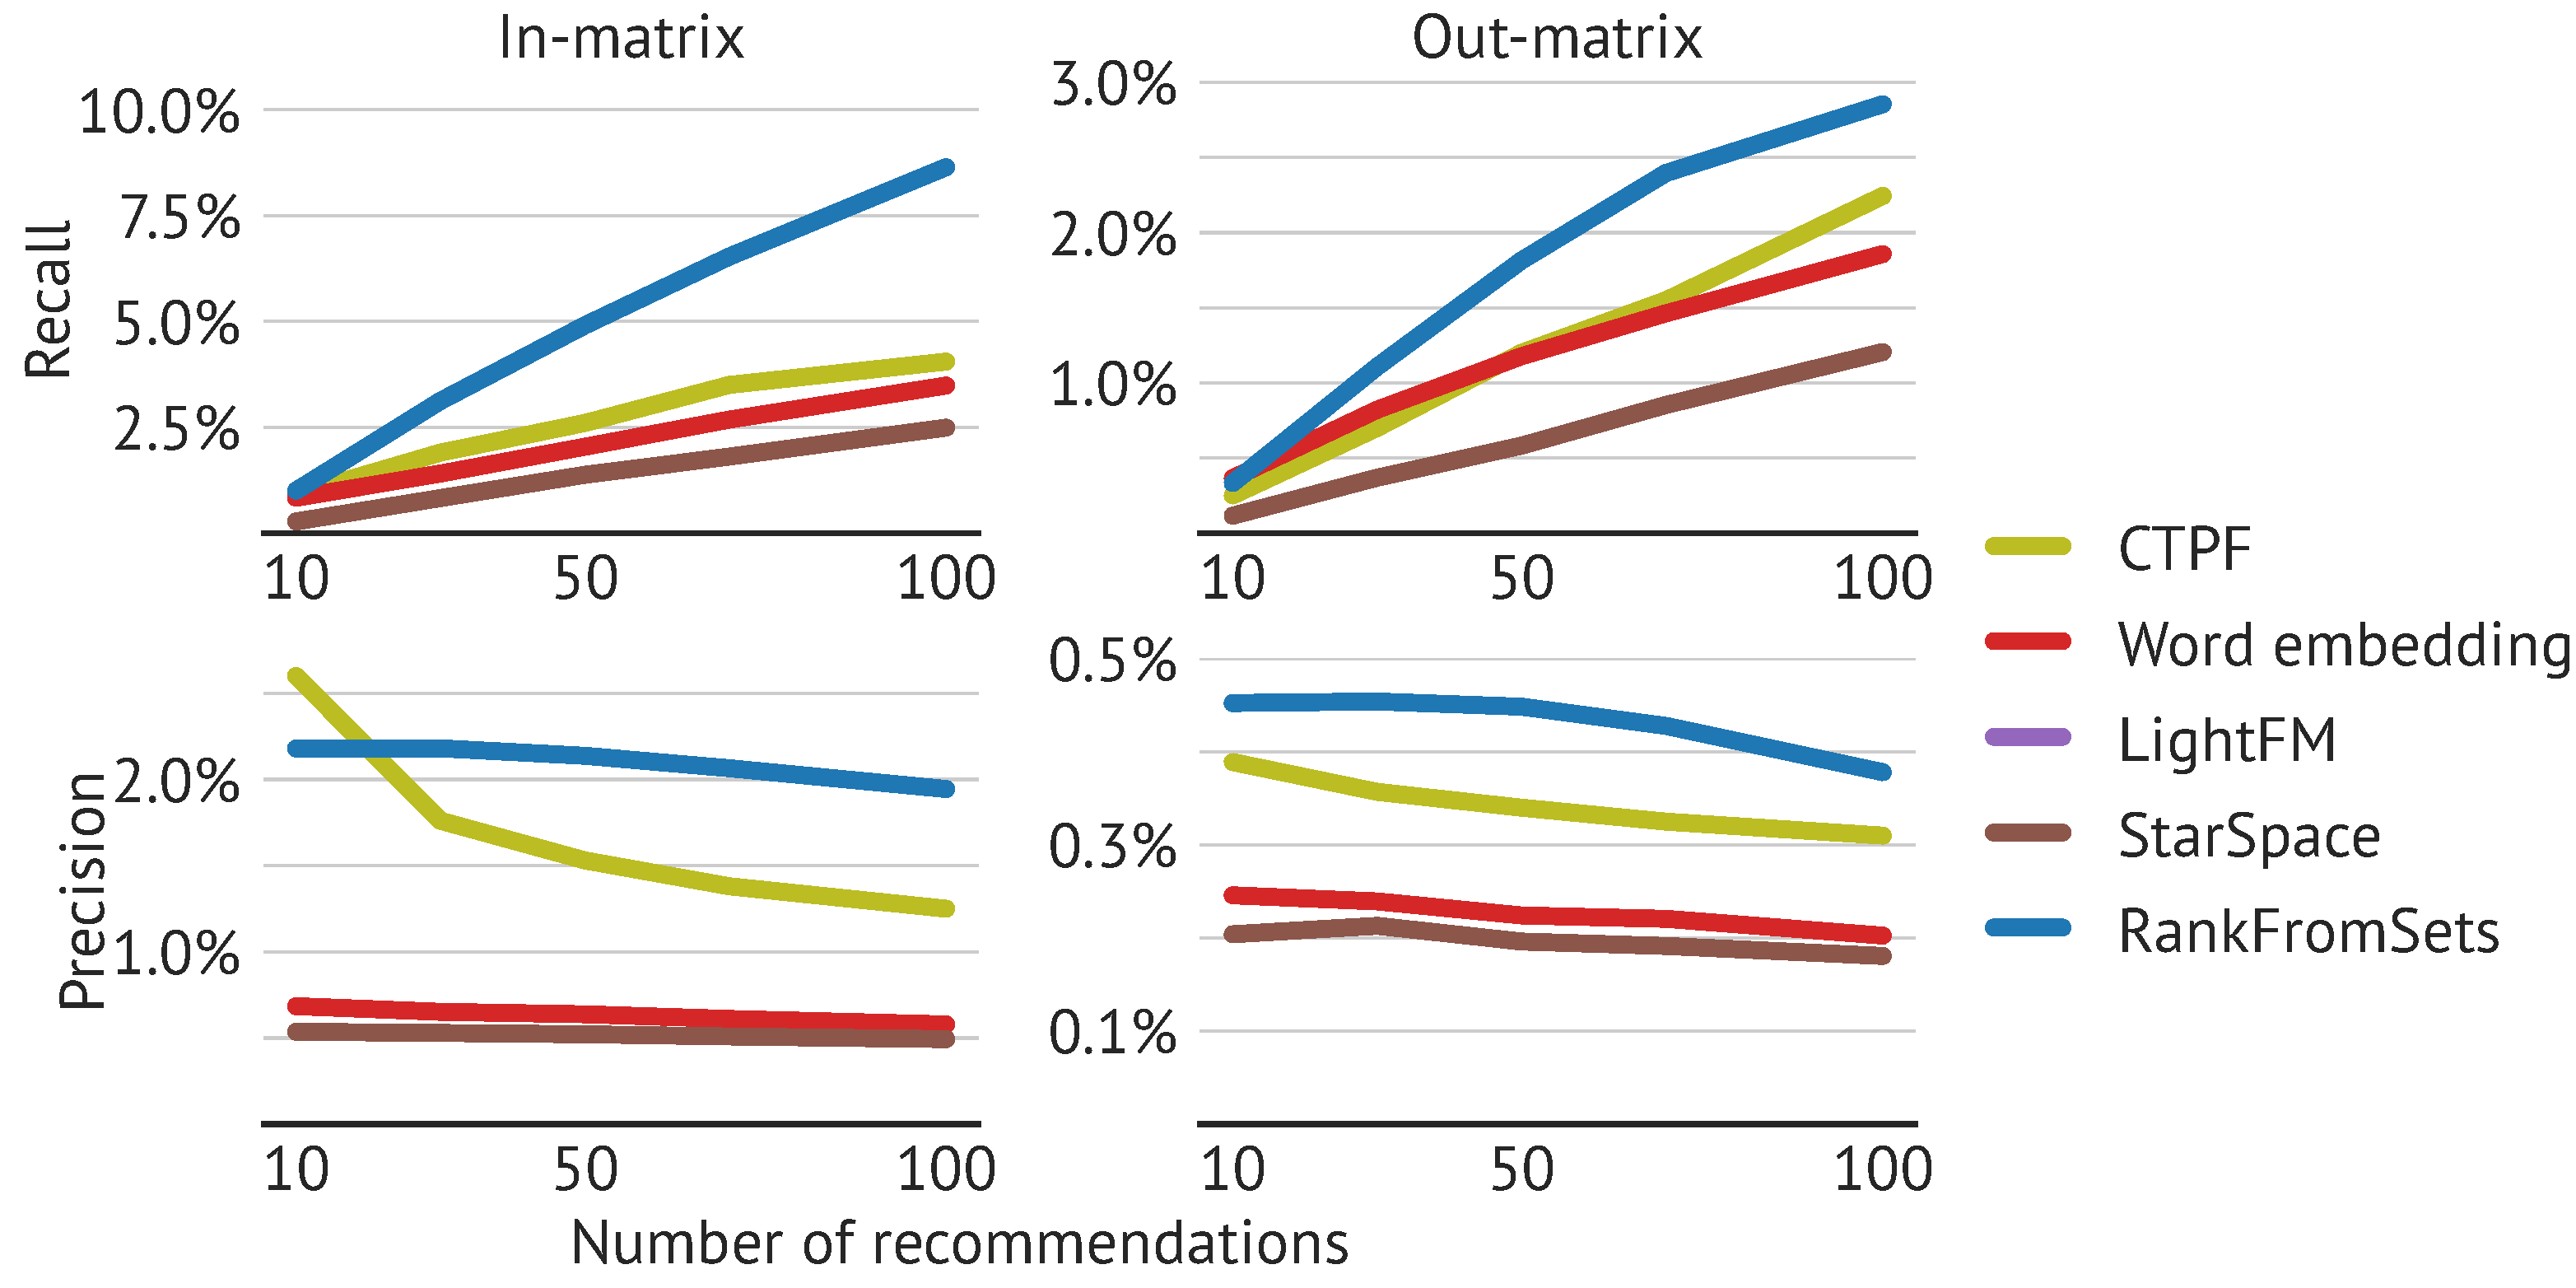
\includegraphics[width=0.7\linewidth]{ch-rfs/fig/arxiv}
\begin{figure*}[t]
  \centering
  \begin{subfigure}{\linewidth}
    \centering
    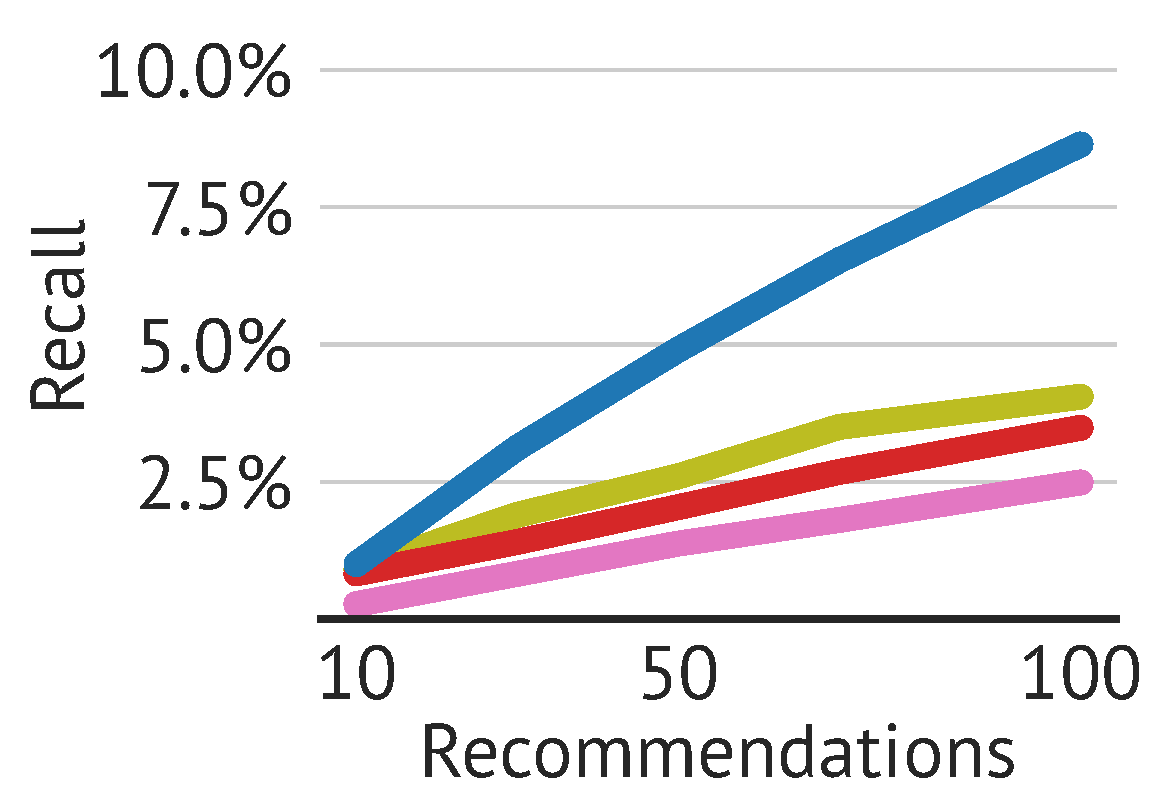
\includegraphics[width=.3\linewidth]{ch-rfs/fig/arxiv-in-matrix-recall}
    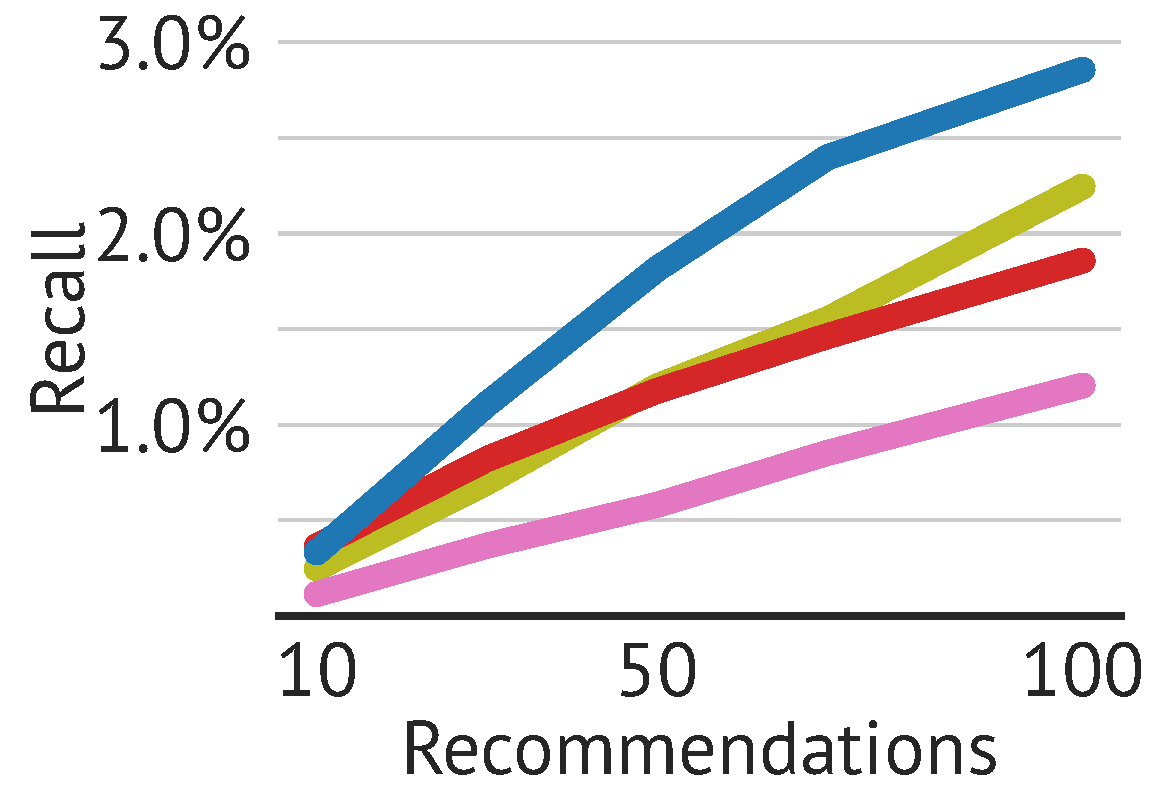
\includegraphics[width=.3\linewidth]{ch-rfs/fig/arxiv-out-matrix-recall}
    \hspace{3mm}
    \raisebox{9mm}{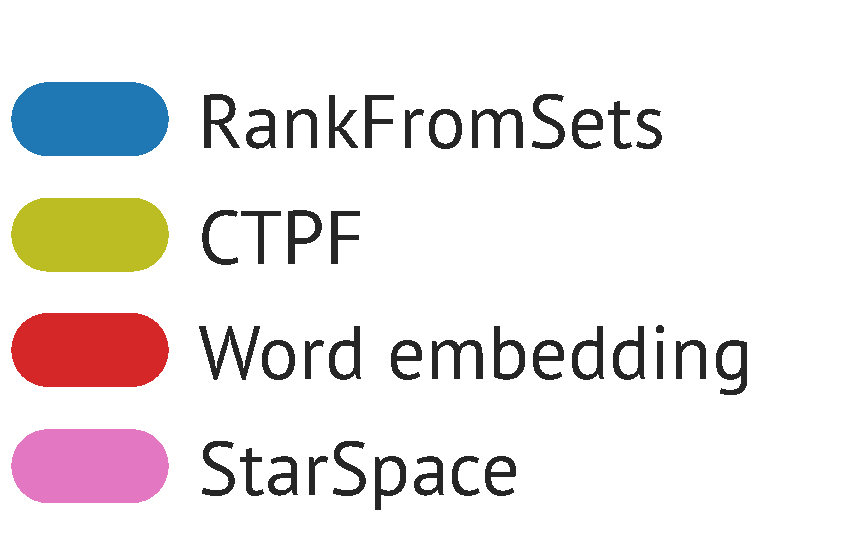
\includegraphics[width=0.2\linewidth]{ch-rfs/fig/arxiv-legend}}
    \caption{Recall for in-matrix (left) and out-matrix (right) documents.}
    \vspace*{0.5cm}
  \end{subfigure}
  \begin{subfigure}{\linewidth}
    \centering
    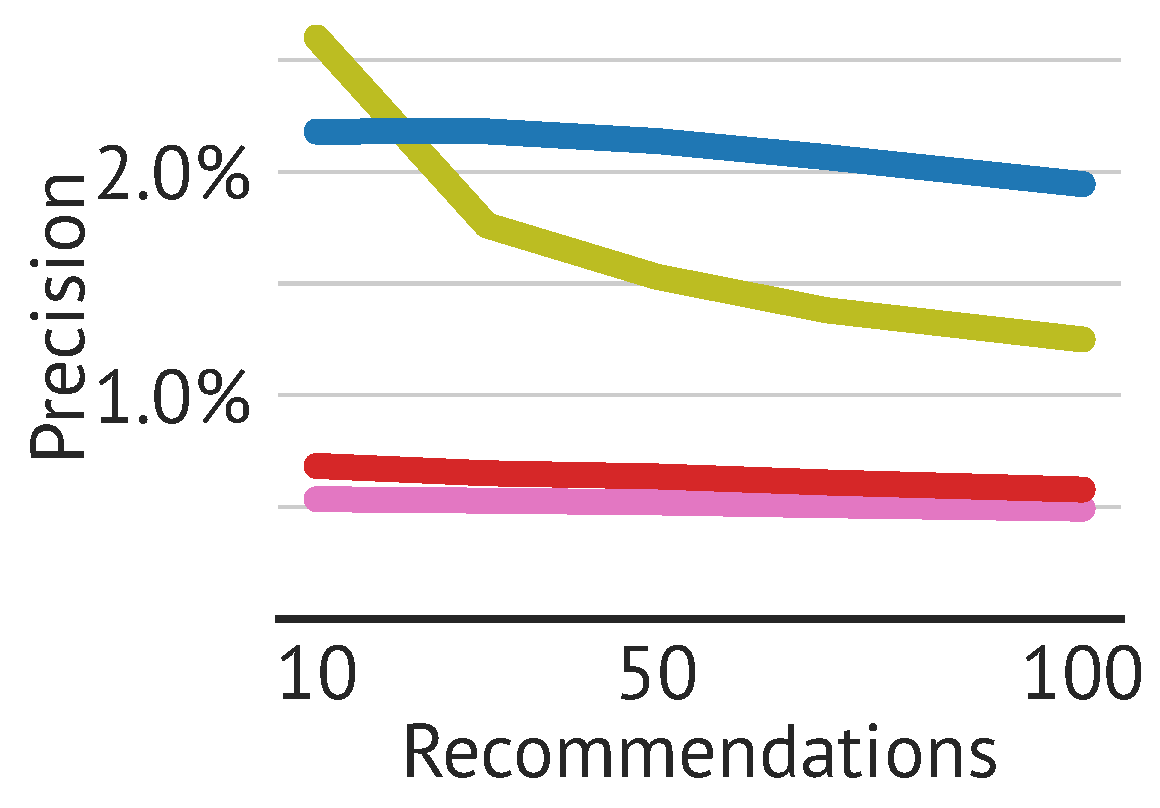
\includegraphics[width=.3\linewidth]{ch-rfs/fig/arxiv-in-matrix-precision}
    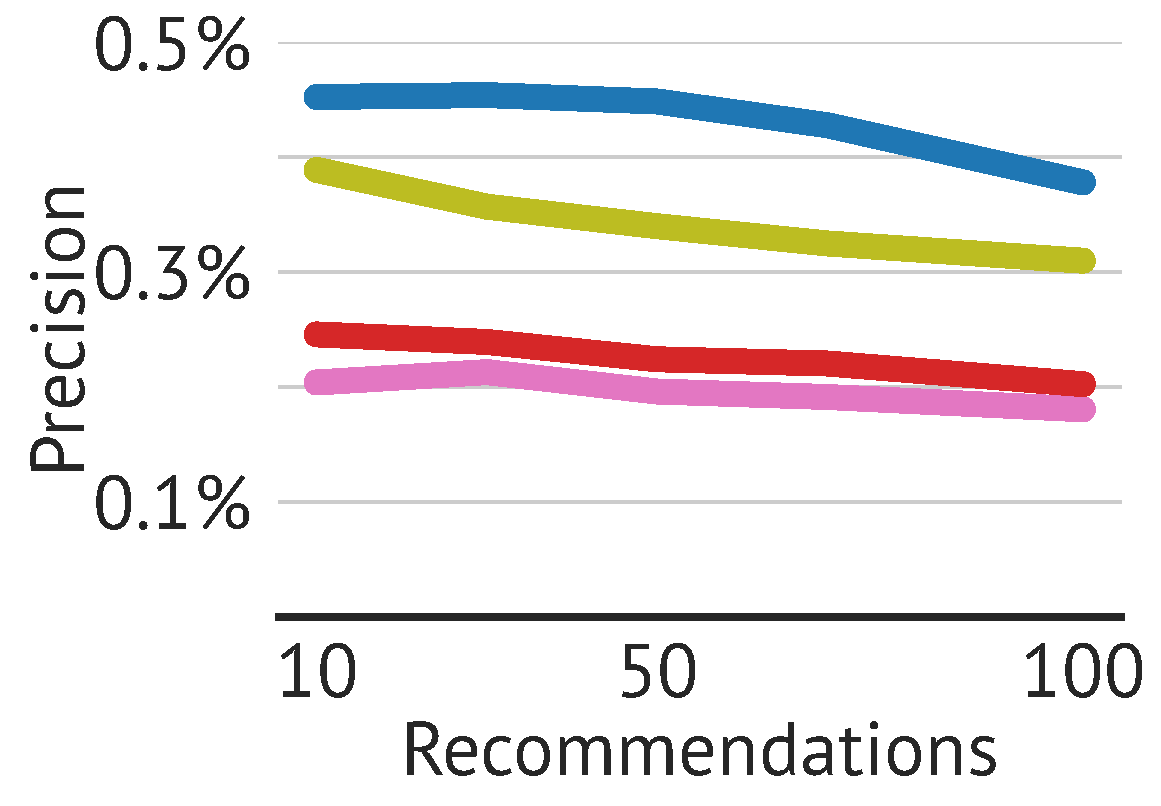
\includegraphics[width=.3\linewidth]{ch-rfs/fig/arxiv-out-matrix-precision}
    \hspace{3mm}
    \raisebox{9mm}{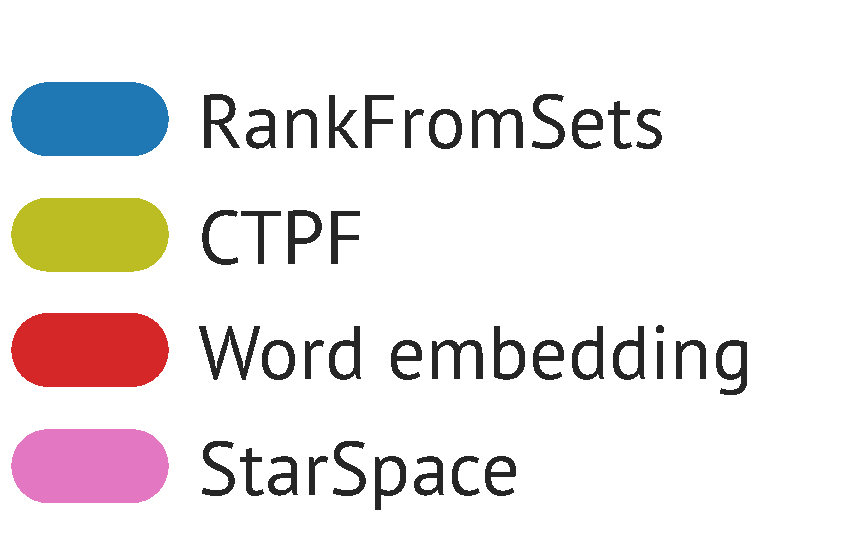
\includegraphics[width=0.2\linewidth]{ch-rfs/fig/arxiv-legend}}
    \caption{Precision for in-matrix (left) and out-matrix (right) documents.}
  \end{subfigure}
  % \begin{subfigure}[b]{\figwidthrfs}
  %   \centering
  %   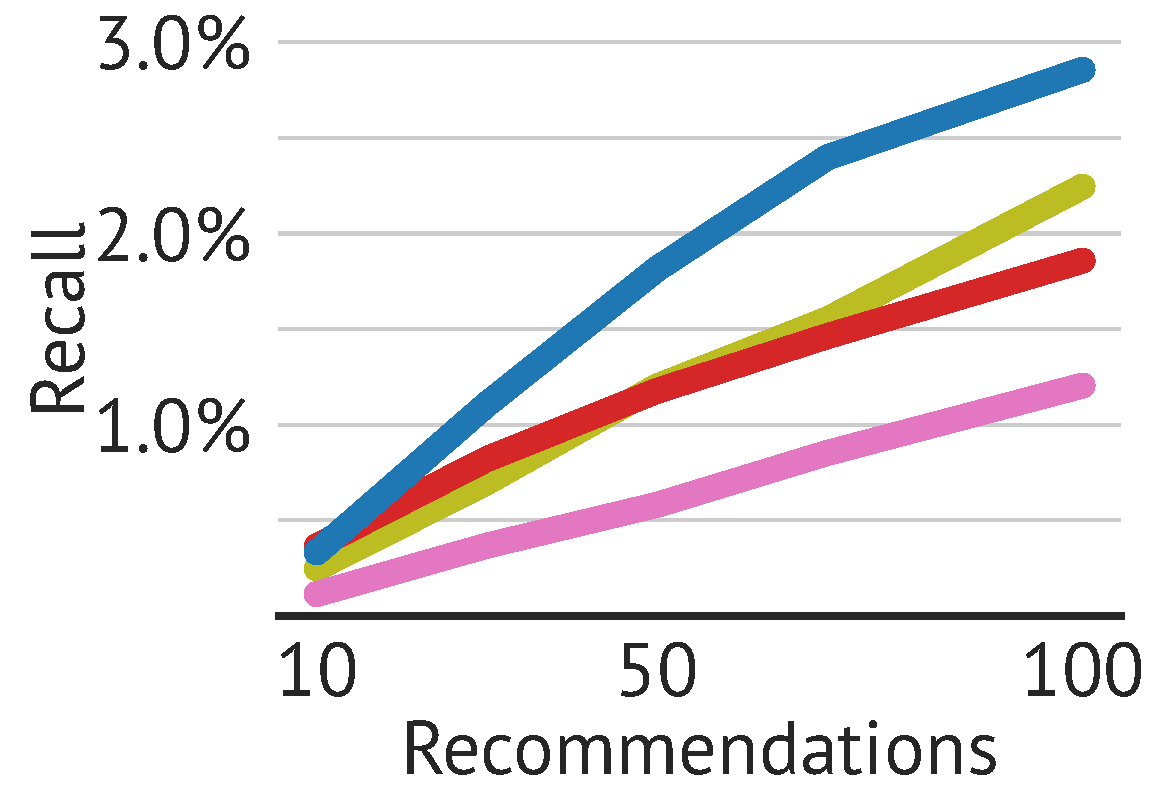
\includegraphics[width=\mysizerfs]{ch-rfs/fig/arxiv-out-matrix-recall}
  %   \caption{Out-matrix}%
  %   \label{fig:arxiv-out-recall}%
  % \end{subfigure}
  % \begin{subfigure}[b]{\figwidthrfs}
  %   \centering
  %   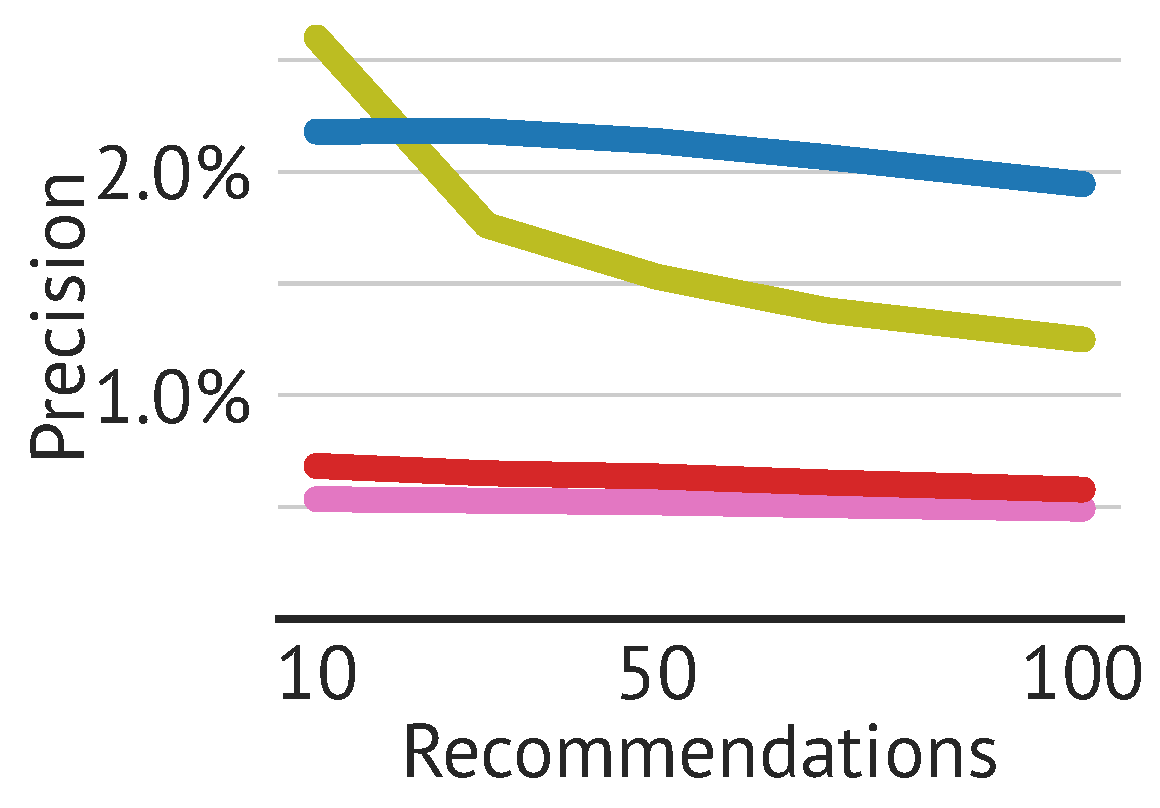
\includegraphics[width=\mysizerfs]{ch-rfs/fig/arxiv-in-matrix-precision}
  %   \caption{In-matrix}%
  %   \label{fig:arxiv-in-precision}%
  % \end{subfigure}
  % \begin{subfigure}[b]{\figwidthrfs}
  %   \centering
  %   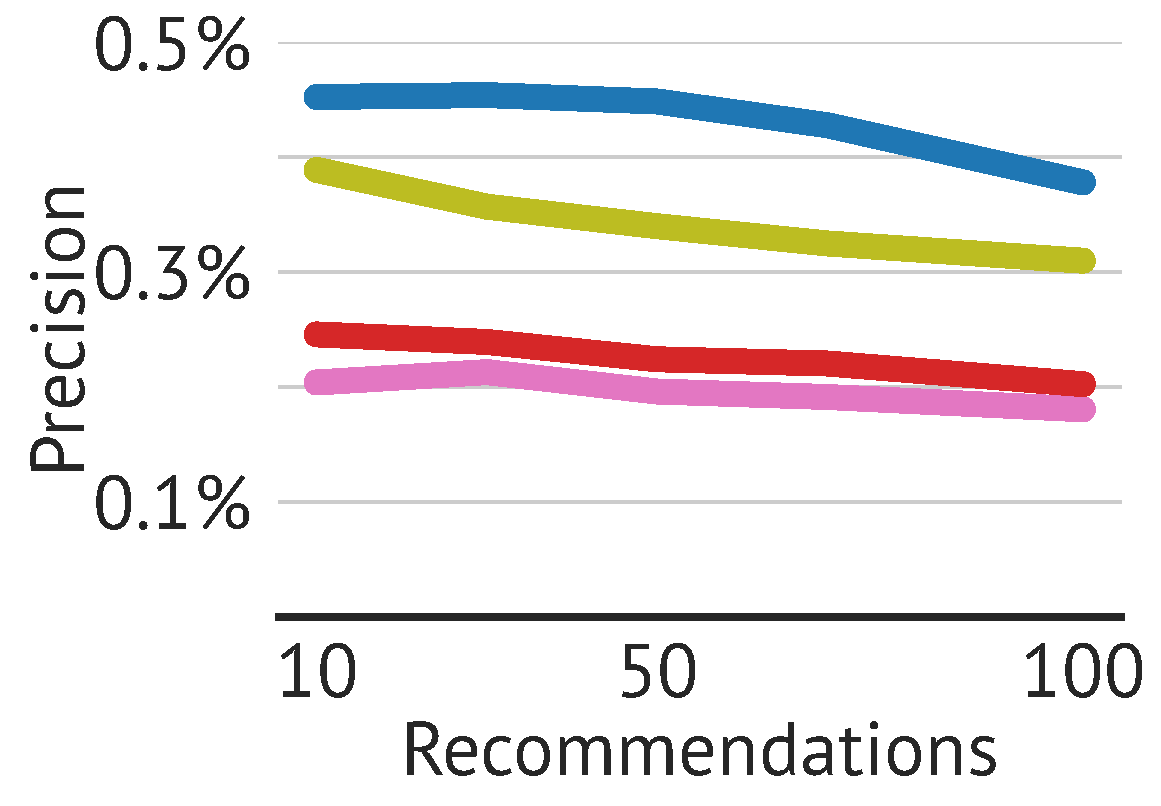
\includegraphics[width=\mysizerfs]{ch-rfs/fig/arxiv-out-matrix-precision}
  %   \caption{Out-matrix}%
  %   \label{fig:arxiv-out-precision}%
  % \end{subfigure}
  \caption[\textsc{rfs} results on arXiv data for article recommendation]{\label{fig:arxiv-performance} \textbf{\acrlong{rfs} outperforms collaborative topic Poisson factorization (\acrshort{ctpf})~\citep{gopalan2014content-based} and other models on recommending arXiv papers to scientists.} The items are documents and the attributes are the unique words in the abstracts. Recommendation performance is evaluated using both precision and recall to match the evaluation in \citep{gopalan2014content-based}. The metrics are reported on training (in-matrix) documents and cold-start (out-matrix) documents with no clicks in the training set. All \acrshort{gru} and \acrshort{lstm}-based models in \citet{bansal2016ask-the-gru:} performed an order of magnitude worse, and these results are omitted (training details are in \Cref{sec:appendix-empirical}).}
\end{figure*}

%As described in \Cref{sec:rfs-experiments}, the unpublished variant of LightFM~\citep{kula2015metadata} with the \acrlong{bpr} objective~\citep{rendle2009bpr:} is equivalent to a classifier. This means it is in the class of \gls{rfs} models and performs equally well (the curves overlap) as anticipated by \Cref {prop:maximizing-recall}.
\Cref{fig:arxiv-performance} shows that models in the \gls{rfs} class outperform others. \gls{rfs} with the inner product parameterization or LightFM with the \gls{bpr} objective have identical performance (as we showed, the \gls{bpr} objective yields a classifier equivalent to \gls{rfs}).  These \gls{rfs} models outperform \gls{ctpf} in terms of in-matrix recall by over $90\%$. \gls{rfs} models also improve over \gls{ctpf} in terms of out-matrix recall, out-matrix precision, and in-matrix precision (for the latter, only when the number of recommendations is greater than $30$). The word embedding model performs comparably to \gls{ctpf} in terms of recall, and performs worse in terms of precision. Recurrent neural network recommendation models were implemented following \citet{bansal2016ask-the-gru:} and given access to full sequence information, unlike \gls{rfs}. (The permutation-marginalized version of these models in \Cref{eq:rnn} is evaluated on meal recommendation where the order of foods in a meal does not carry information.) The training details for the recurrent neural networks are in \Cref{sec:appendix-empirical}, but their performance was an order of magnitude worse than the other methods and these results are omitted. The \gls{rfs} regression function used is in \Cref{eqn:rankfromsets}; the other parameterizations did not fit in GPU memory.

Qualitatively, \gls{rfs} reveals patterns in usage of the arXiv. \Cref{fig:arxiv_tsne} is a dimensionality-reduced plot of the user embeddings that reveals connections between fields of study. Scientists who focus on high energy physics, \texttt{hep}, neighbor specialists in differential geometry, \texttt{math.DG}; these areas share techniques. Machine learning researchers (\texttt{stat.ML} readers) neighbor statisticians (\texttt{math.ST} readers), highlighting the close connection between these fields. Plots for document embeddings show similar patterns. This illustrates how \gls{rfs} captures rich patterns of interaction between users and items, while benefitting from information in the item attributes.

This experiment in recommending research papers also highlights a trade-off in computational budget and desired performance in recommender systems. As described in \Cref{sec:hyper-arxiv}, the recurrent neural network recommendation models in \citet{bansal2016ask-the-gru:} did not perform well with the computational budget allocated for all methods (one day of compute on Tesla P100 GPUs). In further experiments, the performance improved marginally with a larger computational budget of several days. Further research in this domain might compare to transformer models \citep{vaswani2017attention,devlin2019bert:}. Transformers preserve sequence information, unlike \gls{rfs}, although they require large computational budgets to make accurate predictions. This means transformer-based methods may present a different trade-off in recommendation performance than the recurrent neural networks we evaluated in this task.
\paragraph{Recommending Meals.} We evaluate \gls{rfs} on data collected from the LoseIt! diet tracking app. This app enables users to track their food intake to eat healthy. We use a year's worth of data from $55$k active users. This corresponds to $16$M meals, where each meal is comprised of a subset of $3$M foods. To preprocess, we filter the vocabulary by keeping words that occur at least $20$~times in the food names, resulting in $9963$~words. A meal is represented as the union of the sets of words occurring in the food names. For evaluation, 1\% of the items (meals) are held out for evaluating validation and test performance respectively. We evaluate models using SampledRecall@$K$ with $K=10$.

% !TEX root = ../../main.tex
\begin{figure}[t]
  \centering
  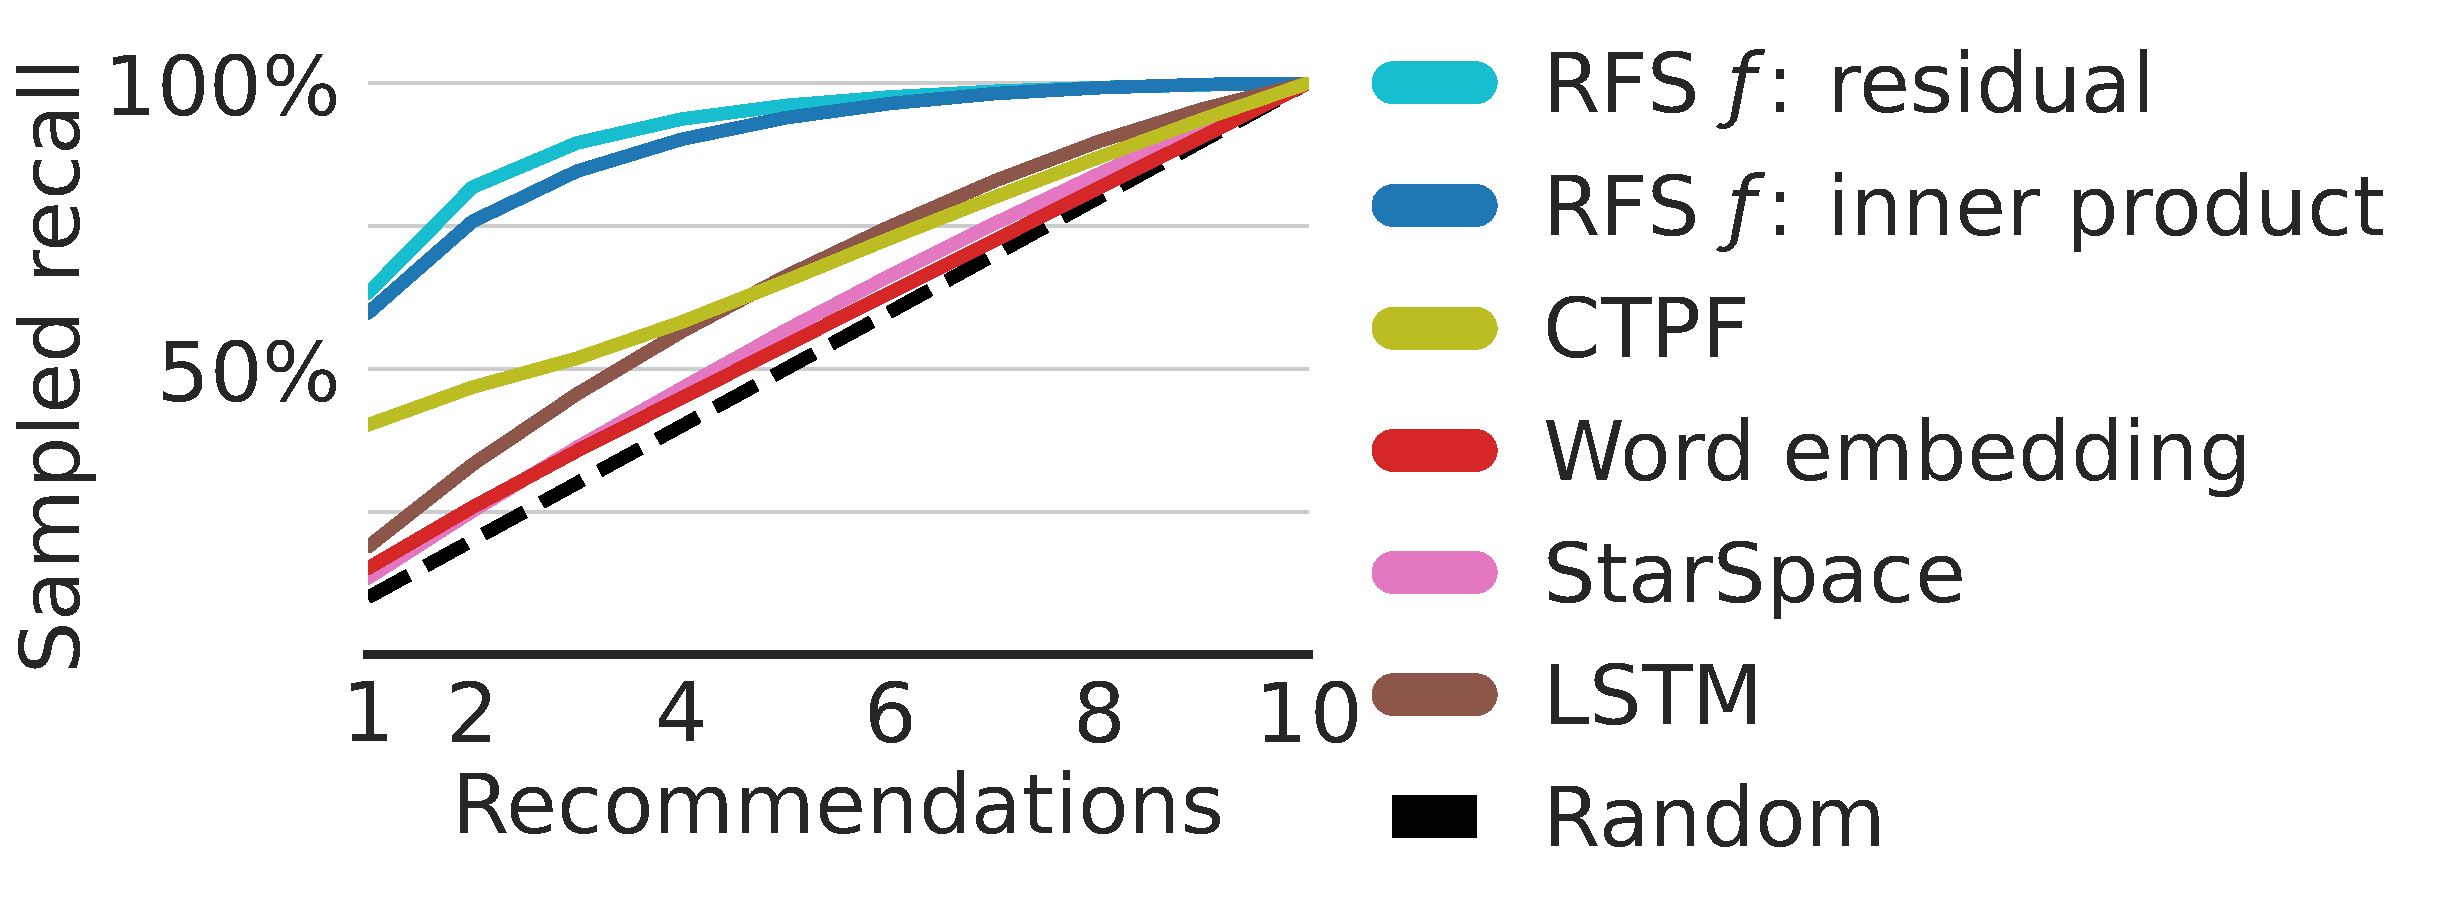
\includegraphics[width=0.7\linewidth]{ch-rfs/fig/meal-recall}
  \caption[\textsc{rfs} results on meal recommendation]{
  \textbf{\acrlong{rfs} models outperform competitors in meal
 recommendation in terms of sampled recall computed using \Cref{eq:sampled-recall}. Comparison models are described in \Cref{sec:models} (see \Cref{sec:appendix-empirical} for hyperparameters). The \gls{rfs} regression functions $f$ are defined in \Cref{eqn:rankfromsets,eqn:neural-network,eqn:residual} for the inner product, neural network, and residual models, respectively.}%
   % % The recommendation models
 % are trained on data from a food
    % tracking app as described in \Cref{sec:experiments_meals} and are evaluated
    % using the sampled recall metric, \Cref{eq:sampled-recall}. The inner
    % product, neural network, and residual regression functions for \acrlong{rfs}
    % are in \Cref{eqn:rankfromsets,eqn:neural-network,eqn:residual}
    }
  \label{fig:meal-recall}
  % \vspace{-0.5cm}
\end{figure}
\Cref{fig:meal-recall} shows the sampled recall: models in the \gls{rfs} class outperform others, such as permutation-marginalized recurrent neural networks and word embedding models. The residual \gls{rfs} model outperforms the \gls{rfs} inner product parameterization (and the equivalent LightFM model trained on the \gls{bpr} objective). The code released with~\citet{gopalan2014content-based} or \citet{wang2011collaborative} did not scale to this size of data, despite sufficient computing resources. This experiment further verifies \Cref {prop:maximizing-recall}: \gls{rfs} models can maximize recall.

Qualitatively, \gls{rfs} learns an interpretable representation of items, as
shown by nearest neighbors of meals in \Cref{tab:nearest_meals}. In this table,
we display breakfast, lunch, and dinner meals, alongside their nearest
neighbors. We find that the nearest neighbors are also breakfast, lunch, and
dinner meals respectively, showing that the attribute embeddings learned by the
model can be used to explore qualitative patterns in the learned latent space.
%%% Local Variables:
%%% mode: latex
%%% TeX-master: "set_recommendation"
%%% End: